\problemname{Tycho}

\illustration{.4}{img/MarsPerseveranceRover.jpg}{}

\noindent
Planētas izpētes transportlīdzeklim \emph{Tycho VIII} pēc minerālu paraugu savākšanas ir jāatgriežas mājas bāzē.
Tycho ceļo pa taisnu līniju no pozīcijas $0$ līdz bāzei, kas atrodas pozīcijā $b$.
Pārvietojoties tas virzās lēnā, bet pastāvīgā tempā ar ātrumu $1$~vienība sekundē.
Katrā sekundē Tycho cieš $1$~vienības vides bojājumus no smagajiem apstākļiem uz planētas.

Situāciju pasliktina tuvējā pulsāra radiācija, kas katru $p$ sekundi izraisa papildus $d$ vienības ar bojājumiem.
Tomēr radiācijas bojājumus var novērst meklējot pajumti vienā no $n$ dažādajiem pa ceļam atrodamajos slēpņos: alās, augsnē, lielos akmeņos, planētas lielo dzīvnieku kaulu karkasos.
Tycho jebkurā punktā var izvēlēties apstāties uz veselu skaitu sekundēm.

Sākuma pozīcija $0$ un bāze $b$ ir ar pajumti, tāpēc Tycho tajās nav pakļauts radiācijas bojājumiem.

\medskip
Kāds ir minimālais bojājumu apjoms, ko Tycho cieš ceļā atpakaļ uz bāzi?

\section*{Piemērs}

Apsveriet situāciju, kad mājas bāze atrodas $18$. pozīcijā un patvērumi ir pozīcijās $8$ un $15$.

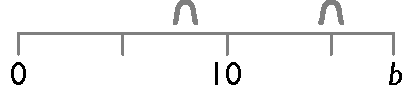
\includegraphics[width=.3\textwidth]{img/samplesetup}

Pieņemsim, ka pulsāra periods ir $4$, tāpēc Tycho bez pajumtes ciestu bojājumus laikos $4$, $8$, $12$ utt.
Ja Tycho atstāj sākuma pozīciju (kurā viņš ir zem pajumtes) laikā $0$, pēc $8$ sekundēm viņš var sasniegt pirmo patvērumu, ciešot radiācijas bojājumus $d$ laika momentā $4$ (bet necieš bojājumus laika momentā $8$, jo tad viņš ir zem pajumtes).
Turpinot bez pārtraukumiem, viņš sasniedz mājas bāzi laikā $18$, ciešot $d+d$ papildu radiācijas bojājumus (laika momentos $12$ un $16$).
Kopumā viņš cieš $d+d+d=3d$ vienības ar radiācijas bojājumiem un $18$ vienības ar vides bojājumiem.
Ja tomēr Tycho gaida $2.$ pajumtē (pozīcijā $15$) $1$ sekundi, impulss laika momentā $16$ viņam nerada nekādus bojājumus, un viņš sasniedz mājas bāzi laikā $19$ ar kopējo bojājumu $2d + 19$ vienības.
Šāds lēmums ir labāks lielākajai daļai $d$ vērtību.
Šeit ir atspoguļotas abas situācijas:

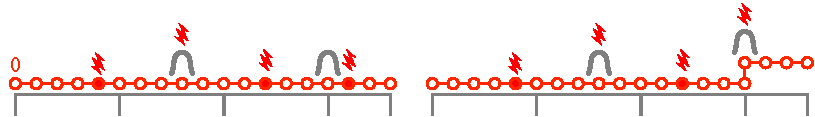
\includegraphics[width=.8\textwidth]{img/sample1_2.pdf}

Ja pulsāra periods ir $10$, Tycho var sākuma pozīcijā gaidīt $2$ sekundes un tad doties uz bāzi bez apstāšanās nevienā pajumtē.
Tādējādi viņš dodas cauri $1.$ patvērumam (pozīcijā $8$) īstajā brīdī, kad pulsārs uzliesmo, un sasniedz mājas bāzi laika momentā $20$, kopumā saņemot $20$ vienības ar vides bojājumiem un nekādus radiācijas bojājumus.

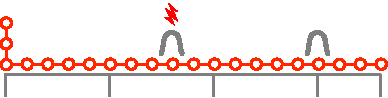
\includegraphics[width=.4\textwidth]{img/sample3.pdf}

\section*{Ievaddati}

Pirmā rinda sastāv no četrām veselām skaitļu vērtībām $b$, $p$, $d$ un $n$, kas ir atdalītas ar vienu atstarpi:
mājas bāzes atrašanās vietu $b$,
pulsāru staru uzliesmojuma periodu $p$,
radiācijas bojājumu apjomu $d$, kuru izraisa katrs pulsāra uzliesmojums,
pajumšu skaits $n$.
Nākamās $n$ rindas satur pa vienam skaitlim, kas apzīmē pajumšu atrašanās vietas $a_1$, $\ldots$, $a_n$, ar nosacījumu, ka
$0<a_1<\cdots <a_n< b$. % constraint:shelterbounds, constraint:sortedshelters

\section*{Izvaddati}

Jāizvada vesels skaitlis - minimālais bojājumu skaits, kas Tycho ir jāuztur, lai sasniegtu punktu $b$.


\section*{Ierobežojumi un vērtēšana}

Jūs varat pieņemt, ka
$p < b$ % constraint:pulsehappens
un
$n < b$. % constraint:sheltersfit
Vienmēr ir spēkā:
$1\leq b\leq 10^{12}$, % constraint:b
$0\leq d \leq 10^6$, %constraint:d
un
$0\leq n \leq 10^5$. % constraint:n

Jūsu risinājums tiks pārbaudīts uz vairākām testu grupām. Katra grupa ir vērta noteiktu punktu skaitu.
Katra testu grupa satur vairākus testus.
Lai saņemtu punktus par testu grupu, ir jāatrisina visi testi testu grupā.
Jūsu gala rezultāts būs lielākais punktu skaits, kas iegūts ar vienu risinājuma iesniegumu.

\medskip
\begin{tabular}{lll}
  Grupa & Punkti & Ierobežojumi\\\hline
  $1$ & $8$  & $p\leq 10^6$ un Tycho nav nepieciešams gaidīt \emph{pēc} pozīcijas pamešanas~$0$.$^*$ \\ % constraint:nowait
  $2$ & $5$  & $b\leq 1000$, $p\leq 100$, $n\leq 10$ \\
  $3$ & $7$  & $b\leq 1000$ \\
  $4$ & $15$ & $p\leq 10^6$, $n\leq 1000$\\
  $5$ & $20$ & $p\leq 100$\\
  $6$ & $35$ & $p\leq 10^6$\\
  $7$ & $10$ & \emph{Bez papildus ierobežojumiem}
\end{tabular}

\medskip
\noindent $^*$ $1.$ testu grupā Tycho var vēl joprojām būt spiests gaidīt pozīcijā $0$ \emph{pirms} tas sāk pārvietoties. Piemēram, $2.$, $3.$ un $4.$ parauga ievaddatos, kas pieder $1.$ testa grupai.
